\begin{figure*}
  \centering
  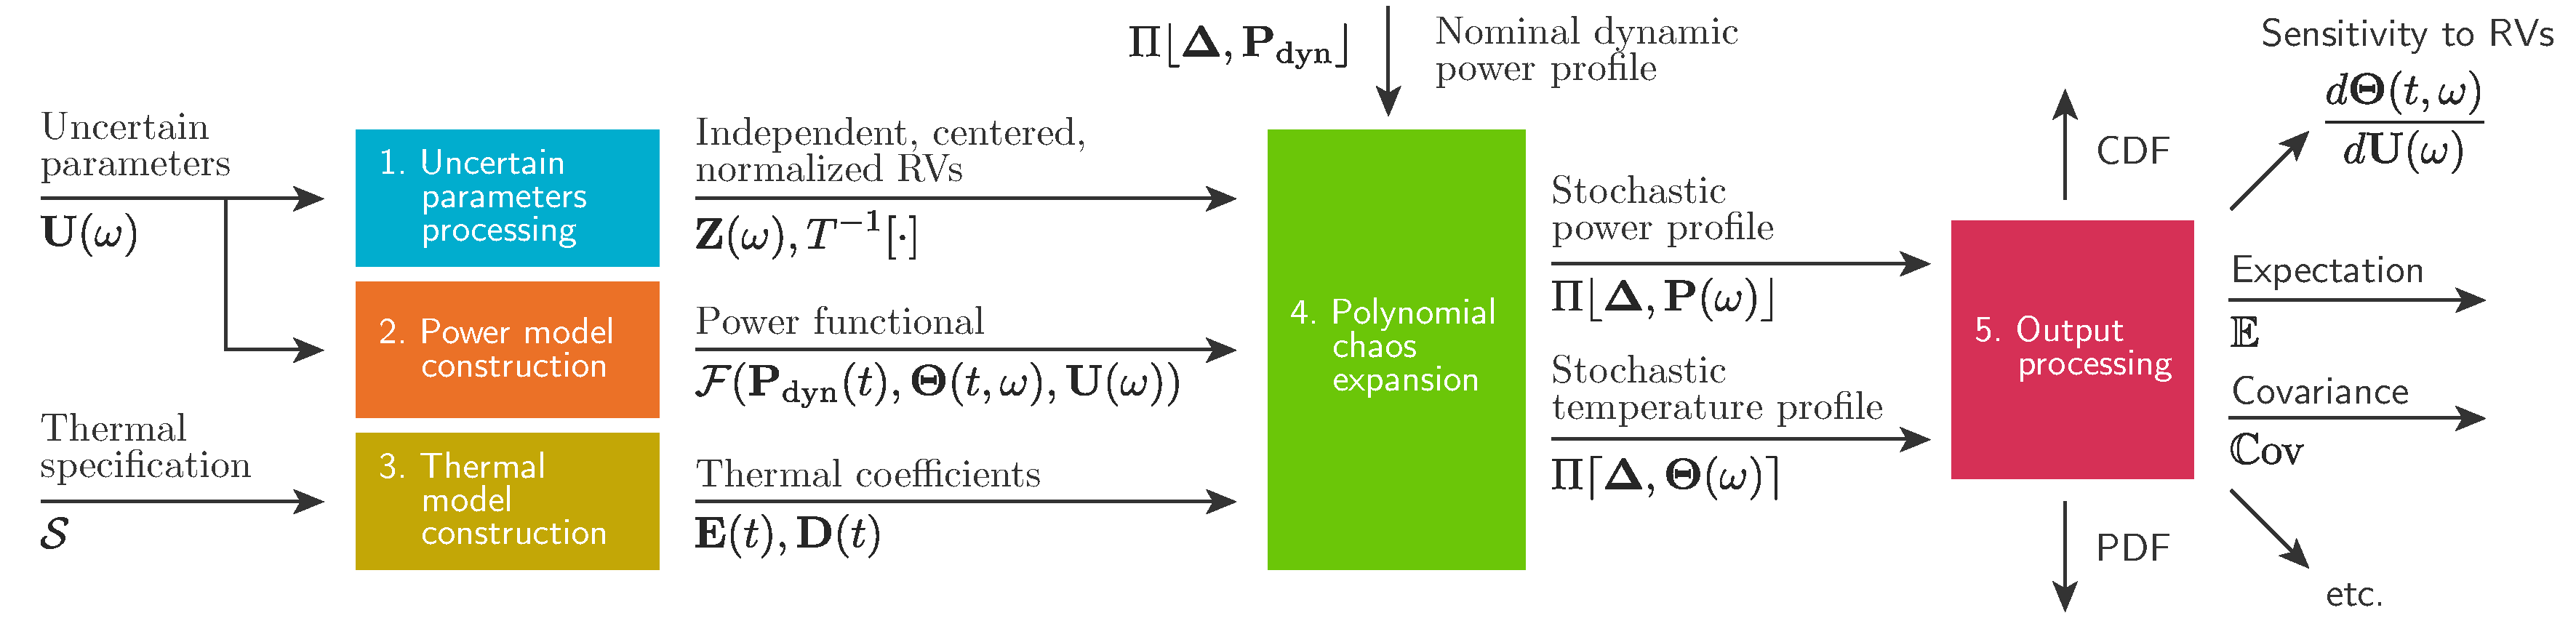
\includegraphics[width=0.9\textwidth]{include/assets/algorithm.pdf}
  \vspace{-0.7em}
  \caption{The structure of the proposed framework.}
  \flabel{algorithm}
  \vspace{-1.6em}
\end{figure*}

The contribution of this paper is in the following: we develop, for the first time, a framework for uncertainty quantification of transient power and temperature variations of multiprocessor systems that depend on a number of uncertain parameters.
The framework is based on the theory of PC expansions, mentioned in \sref{prior-work}, which constitutes an attractive alternative to MC sampling as it possesses much faster convergence properties and is able to construct easy-to-analyze representations of system responses to stochastic inputs.
The proposed framework is flexible in modeling diverse probability distributions, specified by the user, of the parameters, and there are no assumptions on the distributions of the resulting power and temperature traces, as these distributions are unlikely to be known \apriori.
Furthermore, our technique is capable of capturing arbitrary joint effects of the uncertain parameters on the system since the parameters are introduced into the model as a ``black box'', which is also defined by the user.
The framework produces the power and temperature profiles of the system given as polynomials of random variables; the expressions are straightforward to be further analyzed. We will illustrate the framework considering one of the most important parameters affected by process variation: the subthreshold leakage current.
Note, however, that our approach is not bounded to any particular source of variability and, apart from the process-related variations, can be applied to other uncertainties such as those due to the environment, \ie, fluctuations of the supply voltage, ambient temperature, \etc
